\documentclass{article}

\usepackage{packages}
\usepackage[a4paper,left=3cm, right=3cm, top=2cm, bottom=2cm]{geometry} 

\title{\textbf{\LARGE Mappa logistica e caos}\\ {\Large Evoluzione non lineare delle popolazioni}}
\author{Elena Acinapura}
\date{{Università degli Studi di Trento} \\{Dicembre 2019}}


\theoremstyle{teorema}
\newtheorem{teorema}{Teorema}[section]
\theoremstyle{definizione}
\newtheorem{definizione}{Definizione}[section]

\makeindex

\begin{document}
\maketitle
\begin{minipage}{\linewidth}
    \makebox[\linewidth]{
        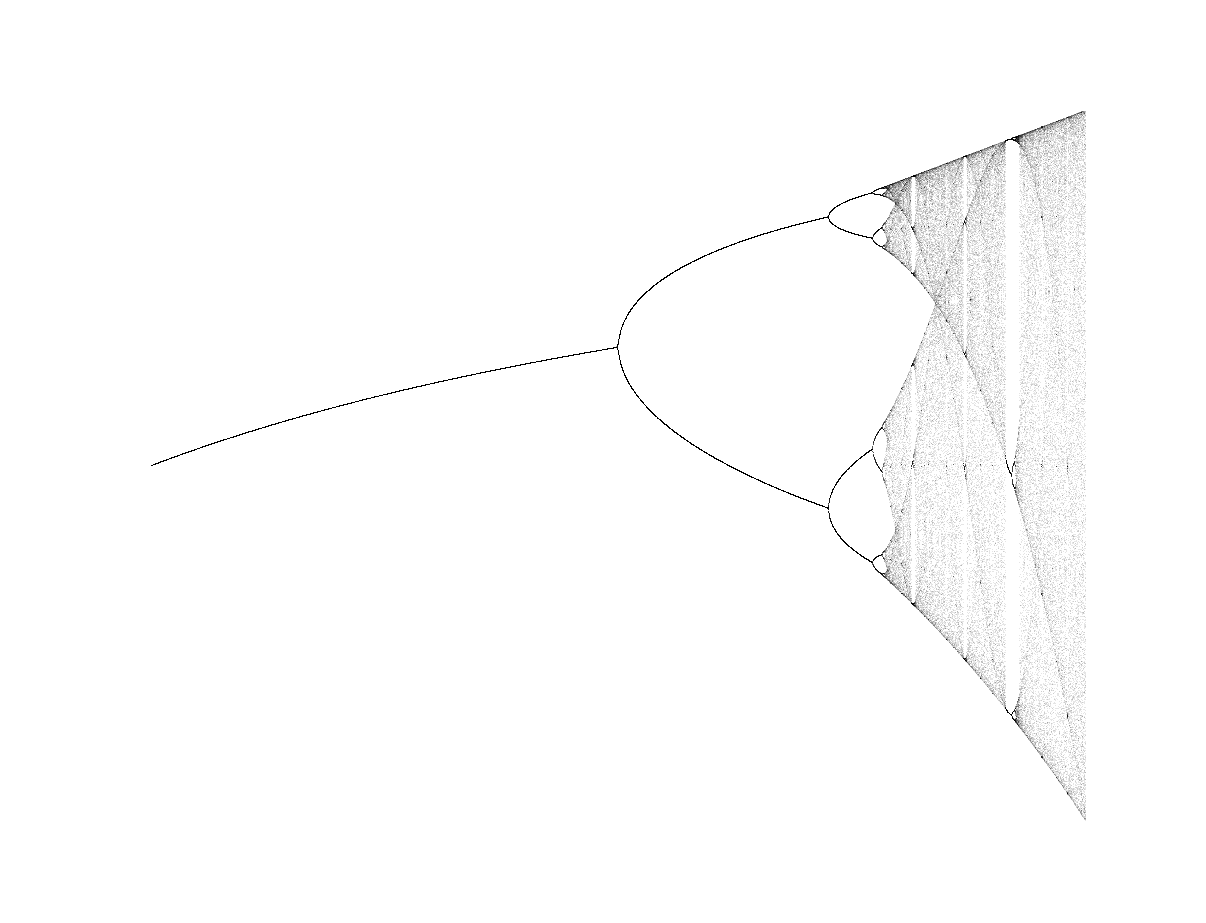
\includegraphics[scale = 0.6]{Immagini/copertina.png}
    }
\end{minipage}

\newpage
\tableofcontents
\newpage

\section{Modelli per l'evoluzione di una popolazione}
\subsection{Descrizione di una popolazione}
Con il termine \textit{popolazione} si intende un insieme di individui in grado di riprodursi, e il cui numero può quindi variare nel tempo. L'interesse principale nello studio della dinamica di una popolazione è trovare dei modelli per come questo numero di individui cambi nel tempo. Dal momento che tale numero è per definizione intero, è comune descrivere il problema in forma discreta, suddividendo il tempo in istanti $t_i$ discreti e indicando con $n_i$ il numero di individui che compongono la popolazione al tempo $t_i$. Formalizzare un modello di evoluzione per la popolazione significa quindi trovare una legge che determina il numero di individui in un dato istante in funzione del numero di individui all'istante precedente, ovvero una funzione $f$ per cui
$$n_{i+1} = f(n_i)$$
Si può inoltre definire il tasso di crescita come il rapporto $$\dfrac{n_{i+1} - n_i}{n_i}$$
L'espressione analitica di $f$ può dipendere in generale da tanti fattori, ma facendo delle semplificazioni e assumendo che la popolazione possa evolvere sotto determinate condizioni, è possibile costruire dei modelli di crescita relativamente semplici, che spesso non sono poi così distanti dalle dinamiche che si riscontrano in molti contesti reali.

\subsection{Evoluzione lineare: il modello di Malthus}
Un primo modello molto semplice per la crescita di una popolazione è quello di Malthus, che ipotizza che la popolazione cresca secondo una relazione lineare con un tasso di crescita $\alpha$ costante, ovvero che
\begin{equation}
    n_{i+1} = n_i + \alpha n_i
    \label{eq:malthus}
\end{equation}
Si vede facilmente che, se $\alpha$ è positivo, la successione {$n_i$} cresce illimitatamente, e in particolare il numero di individui cresce in modo esponenziale: ipotizzando che la popolazione parta da un numero iniziale $n_0 > 0$ e raccogliendo a fattore $n_i$ nel termine generico, si ottiene 
\begin{equation*}
    \begin{gathered}
    n_1 = n_0(1+\alpha) \\ n_2 = n_1(1+\alpha) = n_0(1+\alpha)^2\\\dots \\ n_i = n_0(1+\alpha)^i
    \end{gathered}
\end{equation*}

Questa è la situazione che si verifica in una popolazione in cui i nuovi individui che nascono sono più numerosi di quelli che muoiono, e non vi è nessun ulteriore agente esterno a limitare la crescita della popolazione.

\subsection{Evoluzione non lineare: il modello di Verhulst}
Un avanzamento rispetto al semplice modello di crescita illimitato di Malthus venne proposto da Verhulst: egli ne formulò una correzione che intende tenere conto della limitatezza delle risorse ambientali a disposizione di una popolazione, e introdusse il concetto di \textit{capacità di carico}. L'idea è che la popolazione possa aumentare fino a un numero massimo di individui, $K$, raggiunto il quale le condizioni ambientali ne azzerano la crescita; inoltre, il modello deve prevedere che la velocità di crescità diventi tanto più lenta quanto più il numero di individui si avvicina alla capacità di carico. Verhulst introdusse quindi nell'equazione \ref{eq:malthus} un ulteriore termine dipendente dal rapporto $n/K$ che soddisfi queste richieste, ottenendo
\begin{equation}
    n_{i+1} = n_i + \alpha n_i(1-\frac{n_i}{K})
    \label{eq:verhulst}
\end{equation}
Come si vedrà, questa semplice aggiunta di un termine quadratico alla funzione lineare di Malthus cambia radicalmente l'evoluzione della popolazione, e può renderne la determinazione assai complicata.
\\
Può essere utile riscrivere l'equazione \ref{eq:verhulst} nel seguente modo:
\begin{equation*}
    \begin{gathered}
        n_{i+1} = n_i (1+\alpha+\alpha \dfrac{n_i}{K}) \\
        n_{i+1} =  n_i (1+\alpha) (1- \dfrac{\alpha}{1+\alpha} \dfrac{n_i}{K})
    \end{gathered}
\end{equation*}
Effettuando poi il cambio di variabile
$$x_i = \dfrac{\alpha}{1+\alpha} \dfrac{n_i}{K}$$
 si ottiene 
$$  \cancel{\frac{K (1+\alpha)}{\alpha}} x_{i+1} = \cancel{\frac{K (1+\alpha)}{\alpha}} x_i (1+\alpha) (1- x_i) $$\\
e definendo $r = 1+ \alpha$, si ottiene
\begin{equation}
    x_{i+1} = r x_i (1-x_i)
    \label{eq:logistica}
\end{equation}
L'equazione \ref{eq:logistica} è detta \textit{mappa logistica}, ed è di grande importanza per le sue caratteristiche matematiche, che è intenzione approfondire in queste pagine. Il termine \textit{mappa} indica che la funzione di $x_i$ individuata ha per dominio e codominio lo stesso insieme: in questo caso in particolare, tale insieme è rappresentato dall'intervallo $\left[0,1 \right]$. Da una parte, infatti, valori negativi di $x_i$ non sono ammessi, dato che per definizione il numero di individui di una popolazione è non negativo; dall'altra parte, per valori di $x_i > 1$, il termine successivo $x_{i+1}$ risulterebbe negativo, che nuovamente non è un valore ammissibile. La variabile $x$ si mantiene dunque sempre compresa tra 0 e 1, e può essere vista quindi come una sorta di "normalizzazione" del numero di individui nella popolazione.

L'equazione \ref{eq:logistica} evidenzia inoltre in maniera molto evidente la natura quadratica, e quindi non lineare, della legge di crescita della popolazione; tale non linearità fornisce caratteristiche molto particolari all'evoluzione a partire un certo valore iniziale, e lo scopo delle sezioni successive è quello di studiare le caratteristiche matematiche della mappa logistica al variare del suo parametro descrittivo $r$. Nello specifico si intende approfondire il comportamento asintotico dell'evoluzione prevista dalla mappa logistica, cercando di rispondere in particolare alla seguente domanda: esistono dei valori del numero di individui che, una volta raggiunti, si mantengono costanti nel tempo? Quando esistono, tali punti vengono chiamati \textit{punti fissi}, ed l'intenzione è di studiare quali punti fissi preveda la mappa logistica, quale sia la loro natura e come la loro presenza cambi al variare del parametro $r$. Si vedrà che, in certe circostanze, l'evoluzione asintotica della popolazione presenta un carattere caotico, e si approfondirà in che modo tale carattere si manifesti.


\section{La ricerca dei punti fissi di una popolazione}
Consideriamo una popolazione la cui evoluzione sia descritta dall'equazione logistica \ref{eq:logistica}, che, ricordiamo, è $$ x_{i+1} = r x_i (1-x_i)$$ La domanda più interessante che ci si può porre riguardo alla sua evoluzione è come si comporti il numero di individui normalizzato $x_i$ asintoticamente, ovvero nel limite per $i\rightarrow \infty$. In particolare, ci si chiede se esistano dei valori "di equilibrio", $x_{eq}$, tali che, una volta raggiunti, il risultato delle iterazioni successive si mantenga costante, ovvero tali che $$r x_{eq} (1-x_{eq}) = x_{eq}$$
Tali punti, se esistono, vengono chiamati \textit{punti fissi} dell'equazione logistica.

\subsection{Punti fissi di una funzione e metodo delle iterazioni}
In termini generali, data una funzione $f$,  cercarne i punti fissi significa cercare quei valori di $x$ per cui 
\begin{equation}
    x = f(x)
    \label{eq:punto_fisso}
\end{equation}
Un modo per trovare i punti fissi di una funzione è, naturalmente, quello di risolvere l'equazione \ref{eq:punto_fisso} in modo analitico, quando possibile. Dal momento che questo potrebbe però non essere sempre possibile, un altro metodo per trovare alcuni dei punti fissi di una funzione è il cosiddetto \textit{metodo delle iterazioni}: si parte da un valore $x_0$ scelto arbitrariamente e si calcola $f(x_0) =: x_1$; successivamente si prende $x_1$ e si calcola $f(x_1) =: x_2$. Si prosegue in questo modo, ottenendo una successione definita in modo iterativo:
\begin{equation}
    x_{n+1} = f(x_n)
    \label{eq:ricorsione}
\end{equation}
Se il risultato delle iterazioni tende a stabilizzarsi attorno a un valore, ovvero esiste finito il limite per $n \rightarrow \infty$ di $x_n$, tale valore rappresenta proprio un punto fisso $x_{eq}$ soddisfacente l'equazione \ref{eq:punto_fisso}. Si può intuire che tale metodo non permette di trovare tutti i punti fissi di una funzione, in primo luogo perché il valore trovato asintoticamente potrebbe dipendere dalla scelta iniziare di $x_0$, e in secondo luogo perché il metodo delle iterazioni permette di trovare solo i cosiddetti \textit{punti fissi attrattori}, vale a dire quei valori che sono il limite asintotico delle successioni appena definite. Non si raggiungono infatti i \textit{punti fissi repulsori}, che sono sempre punti soddisfacenti l'equazione \ref{eq:punto_fisso}, ma per i quali si verifica che, se si parte da un valore $x_0$ vicino ad essi, le successioni ricorsive definite in \ref{eq:ricorsione} divergono da essi per andare a convergere verso altri punti fissi (che saranno attrattori). 

Per una popolazione, si può interpretare la differenza tra punti fissi attrattori e repulsori nel modo seguente: se si immagina di perturbare il numero di individui della popolazione spostandolo da un valore di equilibrio, i punti fissi attrattori sono quelli per cui la popolazione si riporta allo stato di equilibrio iniziale, mentre i punti fissi repulsori sono quelli per i quali la popolazione si allontana dal valore di equilibrio iniziale. Si può quindi pensare ai punti fissi attrattori e repulsori come a stati di equilibrio stabili o instabili, in analogia con gli stati di equilibrio dei sistemi fisici. Questa definizione della natura dei punti fissi può essere formalizzata nel seguente modo:
\begin{definizione}{\textnormal{\textbf{Punto fisso attrattivo e punto fisso repulsivo}}}

    Sia $x_{eq}$ un punto fisso di una funzione $f$. $x_{eq}$ è detto \textnormal{punto fisso attrattivo} se, in un intorno di $x_{eq}$, $$\left|f(x_{eq} + \delta x) - f(x_{eq})\right| < \left|\delta x\right|$$
    Viceversa, $x_{eq}$ è detto punto fisso repulsivo se, in un intorno di $x_{eq}$, $$\left|f(x_{eq} + \delta x) - f(x_{eq})\right| > \left|\delta x\right|$$
    \label{def:attrattore_repulsore}
\end{definizione}

Prima di andare a ricavare un criterio per stabilire la natura di un punto fisso, può essere interessante vedere come il metodo delle iterazioni possa essere interpretato graficamente. Rappresentando la variabile $x$ sull'asse delle ascisse e la funzione $f(x)$ sull'asse delle ordinate, il metodo delle iterazioni si traduce nelle seguenti azioni: partendo da un valore iniziale $x_0$, si sale fino a incontrare il punto sul grafico di $f$ di ascissa $x_0$, vale a dire $(x_0, f(x_0)$; l'ordinata di tale punto deve ora diventare l'ascissa della successiva iterazione, quindi si può tracciare la bisettrice e, partendo dal punto trovato, muoversi orizzontalmente verso di essa, dove si incontrerà il punto $(f(x_0), f(x_0))$. Si può ora ripetere la procedura partendo da questo punto, muovendosi verticalmente fino a incontrare il punto $\left(f(x_0 ) , f(f(x_0)) = x_1 \right)$, muovendosi poi verso la bisettrice, e avanti così. Si osserverà che questo metodo permette di convergere a un punto fisso di $f$, che si troverà all'intersezione tra il grafico di $f$ e la bisettrice. Si può inoltre osservare che ci sono alcuni punti che, pur essendo intersezioni tra il grafico e la bisettrice, non sono mai il limite asintotico del metodo delle iterazioni: sono punti fissi repulsori.

Nella figura \ref{fig:iterazioni} è presente un esempio con $f(x) = x^2$. Si può osservare che i punti fissi sono $x = 0$ e $x=1$, come si ricava facilmente in modo analitico, che sono infatti i punti di intersezione tra la parabola e la bisettrice. Inoltre sono state rappresentate alcuni iterazioni partendo da valori iniziali diversi, che permettono in particolare di vedere come non importa quanto vicino a $x=1$ inizino le iterazioni, non si converge mai a $x = 1$, punto fisso repulsore.

\begin{figure}[h!]
    \begin{center}
    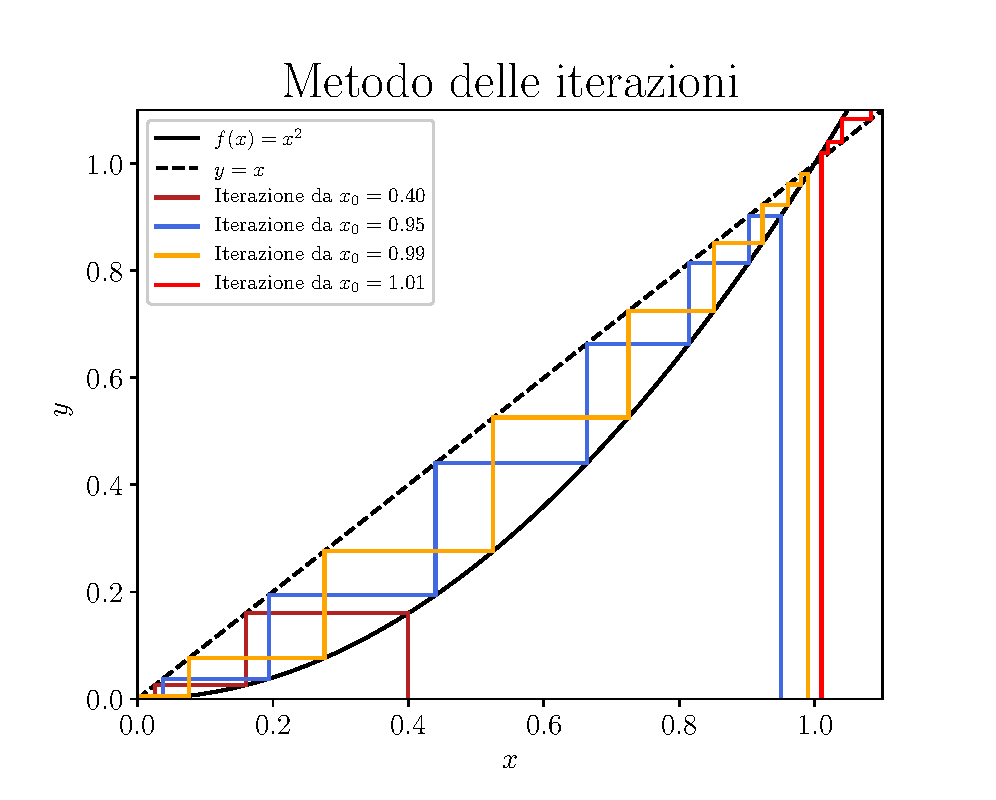
\includegraphics[scale=0.7]{Immagini/iterazioni.eps}
    \captionsetup{width=.8\linewidth}
    \caption{I punti fissi di $f(x) = x^2$ sono le intersezioni tra la funzione e la bisettrice. Il metodo delle iterazioni applicato ad $f$ mostra che le iterazioni convergono sempre a $x=0$, punto fisso attrattore, se si parte da un valore iniziale $0<x_0<1$. Se si parte invece da un valore $x_0 > 1$ le iterazioni divergono all'infinito. Il punto fisso $x=1$ invece non viene mai raggiunto, per quanto vicino vi si parta, ed è infatti repulsore.}
    \label{fig:iterazioni}
    \end{center}
\end{figure}


\subsection{Un criterio per stabilire la natura dei punti fissi}
Come è possibile, in generale, sapere se una funzione ammette punti fissi, e, nel caso in cui questi siano ricavabili per via analitica o per successioni, come è possibile stabilirne la natura? Fortunatamente, per quanto riguarda l'esistenza di punti fissi, un teorema qui non dimostrato ne assicura l'esistenza per tutte le funzioni continue definite da un insieme chiuso in se stesso. Per quanto riguarda invece la determinazione della natura dei punti fissi, il seguente teorema fornisce un criterio per stabilire la repulsività o attrattività dei punti fissi di una funzione, che in molti casi risulta di utile applicazione.

\begin{teorema}
Sia $A\subset \mathbb{R}$ chiuso, sia $f : A \rightarrow A$ una funzione derivabile in A e sia $x_{eq}$ un punto fisso per f. Allora $x_{eq}$ è un punto fisso attrattore per $f$ se e solo se 
\begin{equation}
    \left| \dfrac{\dif f(x)}{\dif x}\right| _{x_{eq}} < 1
    \label{eq:attrattore}
\end{equation}
Viceversa, $x_{eq}$ è un punto fisso repulsore per $f$ se e solo se
\begin{equation}
    \left| \dfrac{\dif f(x)}{\dif x}\right| _{x_{eq}} > 1
    \label{eq:repulsore}
\end{equation}
\label{teorema}
\end{teorema}
\begin{proof}[Dimostrazione]
    
    Dimostriamo la condizione \ref{eq:attrattore} per un attrattore, quella per un repulsore è analoga. Richiamiamo la definizione di punto fisso repulsore data nella Definizione \ref{def:attrattore_repulsore}:
    $$|f(x_{eq} + \delta x) - f(x_{eq})| < |\delta x|$$
    Dal momento che $f$ è derivabile, si può sviluppare al prim'ordine la funzione attorno a $x_{eq}$
    $$ |\delta x| \left| \dfrac{\dif f(x)}{\dif x} \right|_{x_{eq}} + o(|\delta x|) < |\delta x|$$
     dividendo per $|\delta x|$ e facendo il limite per $\delta x \rightarrow 0$ si ottiene infine
    $$ \left| \dfrac{\dif f(x)}{\dif x}\right| _{x_{eq}} < 1$$
\end{proof}

\section{Studio dei punti fissi della mappa logistica}
Una volta visto cosa rappresentano i punti fissi di una funzione e alcune loro caratteristiche, si può finalmente tornare al problema della descrizione della dinamica di una popolazione, e cercare i punti fissi della mappa logistica scelta per descriverla. Allo scopo di analizzarla con più facilità dal punto di vista analitico, può essere comodo d'ora in poi scrivere l'equazione logistica in forma continua, vale a dire nella forma
\begin{equation}
    f(x) = rx(1-x) = rx - rx^2
    \label{eq:logistica_continua}
\end{equation}
Si tratta dunque di una famiglia di infinite funzioni, che dipendono dal parametro $r$. Nella figura \ref{fig:logistiche} sono state rappresentate alcune di queste funzioni al variare di $r$.

Da un punto di vista rigoroso l'operazione di rendere continua la mappa logitica discreta deve essere fatta con cautela, dal momento che i valori di $x$, nel caso di una popolazione composta da un numero intero di invidui, possono essere razionali ma non irrazionali. Dal punto di vista della trattazione, tuttavia, lavorare con funzioni definite sui reali permette di usare gli strumenti dell'algebra e dell'analisi che sono di grande utilità. Si studierà quindi il comportamento dell'equazione logistica da un punto di vista più astratto, tenendo presente queste osservazioni nel caso in cui si intendano applicare i risultati ad una vera popolazione.\\
\begin{figure}[h!]
    \begin{center}
    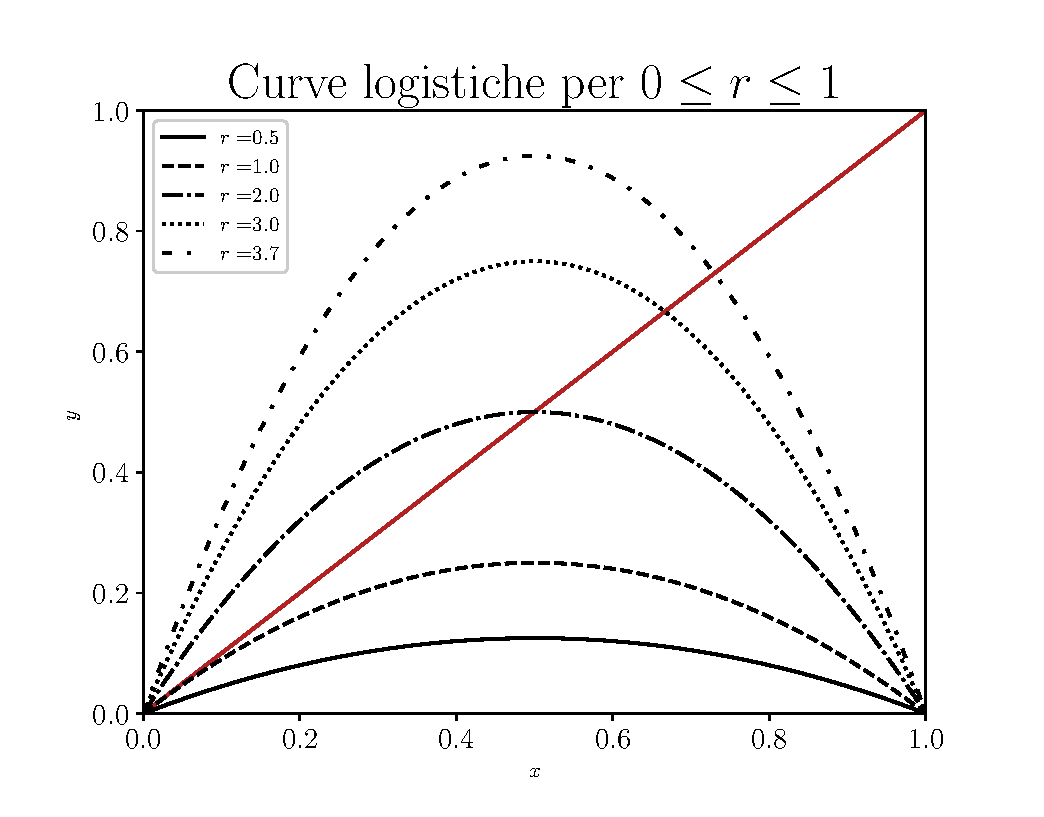
\includegraphics[scale=0.65]{Immagini/curve_logistiche.eps}
    \captionsetup{width=.8\linewidth}
    \caption{Curva logistica per diversi valori del parametro $r$. È stata tracciata anche la bisettrice in rosso, che sarà utile per individuare i punti fissi.}
    \label{fig:logistiche}
    \end{center}
\end{figure}

Si vuole dunque studiare quali sono i punti fissi della funzione \ref{eq:logistica_continua} nell'intervallo di interesse $[0,1]$ al variare del parametro $r$. Innanzitutto bisogna osservare che, se il valore di $f$ deve rimanere all'interno dell'intervallo $[0,1]$, $r$ non può ammettere valori arbitrari. Dalla figura \ref{fig:logistiche} si osserva che il valore massimo assunto dalla funzione logistica dipende dal valore di $r$ e si trova in corrispondenza del vertice; calcolando che l'ordinata del vertice corrisponde a $r/4$, e imponendo che questo sia compreso tra 0 e 1 (inclusi, dato che gli estremi sono valori ammessi), si ottiene la condizione 
\[
    \boxed{0 \leq r \leq 4}
\]
Una volta appurato ciò, si possono calcolare facilmente i punti fissi della funzione \ref{eq:logistica_continua} risolvendo in modo algebrico l'equazione $$ x = rx - rx^2$$ le cui soluzioni generali sono 
\[
    \boxed{x_{eq,1} = 0} \quad \boxed{x_{eq,2} = 1 - \dfrac{1}{r}}
\]
L'interesse è ora quello di studiare la natura di questi punti fissi al variare di $r$. A tal fine, può essere utile riportare qui anche la funzione derivata di f, che verrà utilizzata più volte in seguito:
\begin{equation}
    \dfrac{\dif f(x)}{\dif x} = r (1-2x)
    \label{eq:derivata}
\end{equation}
\subsection{Punti fissi per $0\leq r \leq 1$}
Per valori di $r$ compresi tra 0 e 1, $x_{eq,2}$ risulta minore di 0, dunque non è un valore ammesso e si considera soltanto il punto fisso $x_{eq,1} = 0$. Si osservi che, graficamente, questo si traduce nell'avere un solo punto di intersezione tra la curva logistica e la bisettrice nell'intervallo di interesse, come si verifica nella figura \ref{fig:logistiche_r_minore_1}. 
\begin{figure}[h!]
    \begin{center}
        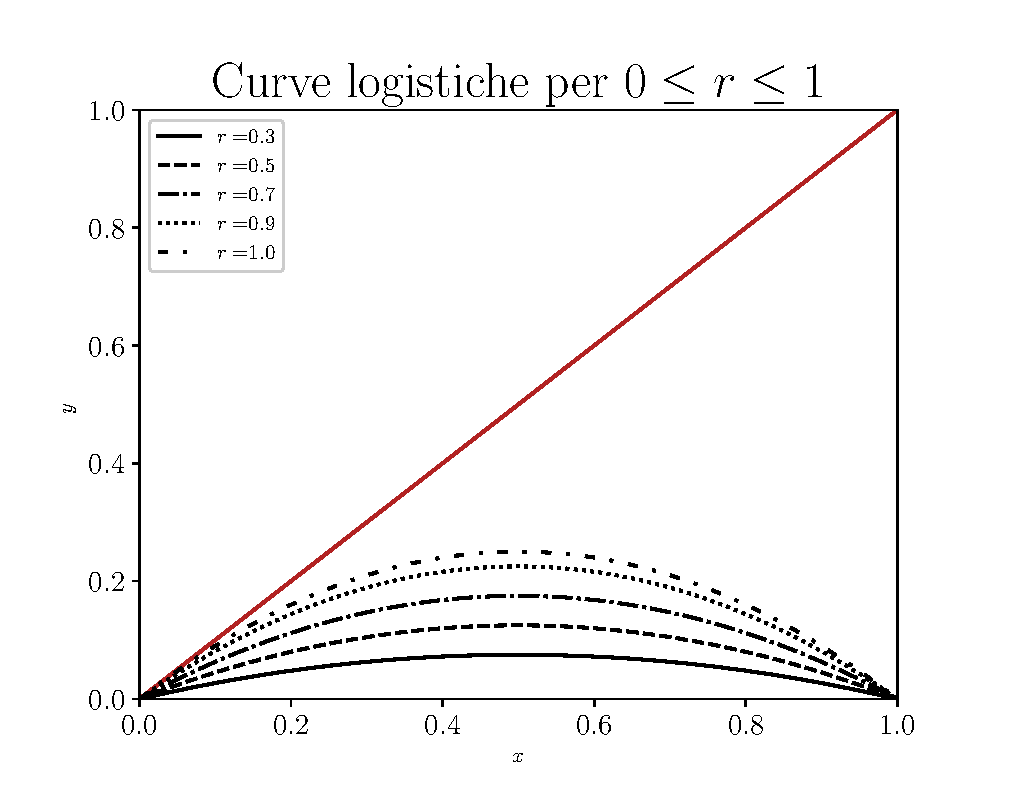
\includegraphics[scale=0.7]{Immagini/curve_logistiche_r_minore_1.eps} 
    \captionsetup{width=.8\linewidth}
    \caption{Diverse curve logistiche per $0\leq r \leq 1$. Si osserva in particolare che c'è una sola intersezione tra le curve e la bisettrice, $x = 0$, che è l'unico punto fisso per i valori considerati di $r$.}
    \label{fig:logistiche_r_minore_1}
    \end{center}
\end{figure}

La derivata di $f$ calcolata in $x = 0$ risulta essere pari a $r$. Per $r < 1$ si ha quindi la certezza che $x_{eq,1} = 0$ sia un punto fisso attrattore, come è ragionevole supporre se si pensa che per $r<1$ la popolazione non può che diminuire a ogni iterazione, fino a estinguersi. Non è possibile usare il metodo della derivata per $r = 1$ invece, ma ci si rende facilmente conto che iterando la funzione $f(x) = x - x^2$ partendo da valori di $x$ compresi tra 0 e 1, si ottiene una successione decrescente di valori convergente a 0; quindi $x_{eq,1} = 0$ è punto fisso attrattivo anche per $r = 1$. Nella figura \ref{fig:r1} si possono osservare diverse successioni per $r=1$ partendo da diversi valori di $x$, tutte convergenti a 0.

\begin{figure}[h!]
    \begin{center}  
    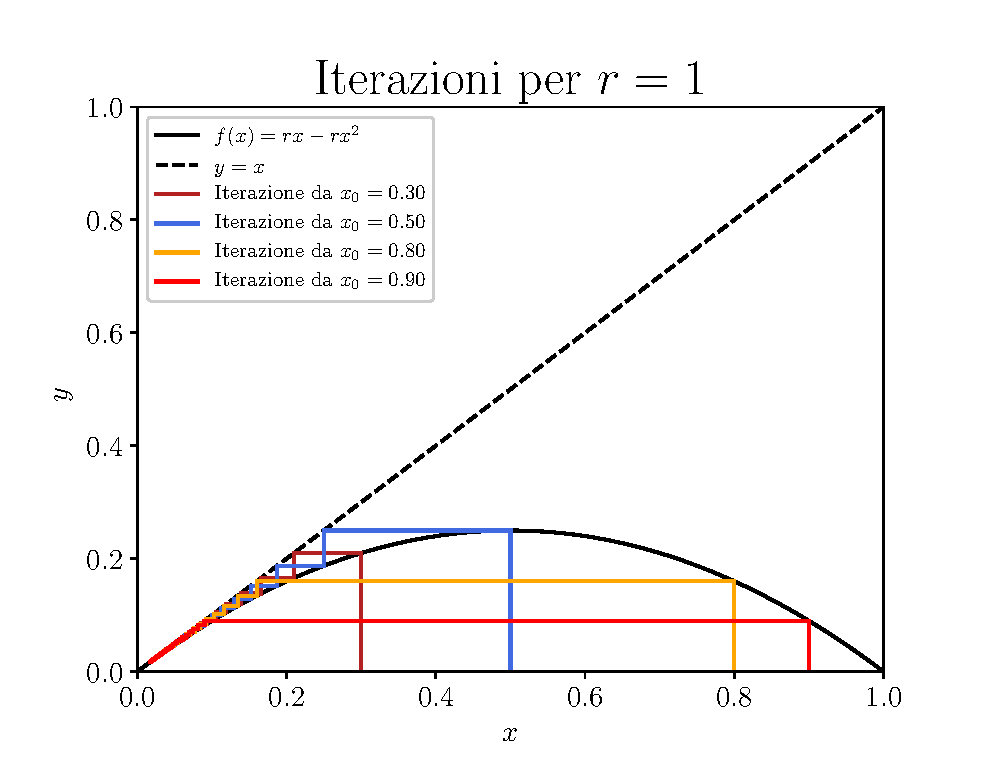
\includegraphics[scale=0.7]{Immagini/iterazioni_r1.eps} 
    \captionsetup{width=.8\linewidth}
    \caption{Iterazioni della funzione logistica per $r=1$, a partire da diversi valori iniziali, convergono sempre a 0.}
    \label{fig:r1}
    \end{center}   
\end{figure}

\subsection{Punti fissi per $1 < r \leq 3$}
Per $1 < r < 3$, il punto fisso $x_{eq,1} = 0$ diventa un punto fisso repulsivo: infatti la derivata di $f$ in $x_{eq,1}$, come si è visto, vale $r$, che ora è maggiore di 1.

Adesso, inoltre, il valore dell'altro punto fisso $x_{eq,2} = 1 - 1/r$ è un valore ammissibile, e si può studiarne la natura. La derivata di $f$ calcolata in $x_{eq,2}$ vale $$ \left.\dfrac{\dif f(x)}{\dif x}\right\vert_{x_{eq,2}} = 2 -r$$ 
che risulta sempre minore di 1 in valore assoluto per $1 < r < 3$, quindi $x_{eq,2}$ è ora un punto fisso attrattore. 
Il caso $r=3$ non è risolvibile tramite lo studio della derivata, perché presso $x_{eq,2}$ essa vale $-1$. Attraverso il metodo delle iterazioni si trova che le successioni convergono sempre verso $x_{eq,2}$, ma con estrema lentezza. Nella figura \ref{fig:r3} è stato raffigurato il risultato del metodo delle iterazioni applicato ad $f$ con $r=3$ dopo 1000 iterazioni, dove si osserva che nonostante l'elevato numero di iterazioni, ancora si distinguono lo stato del sistema e punto di convergenza.
\begin{figure}[h!]
    \begin{center}  
    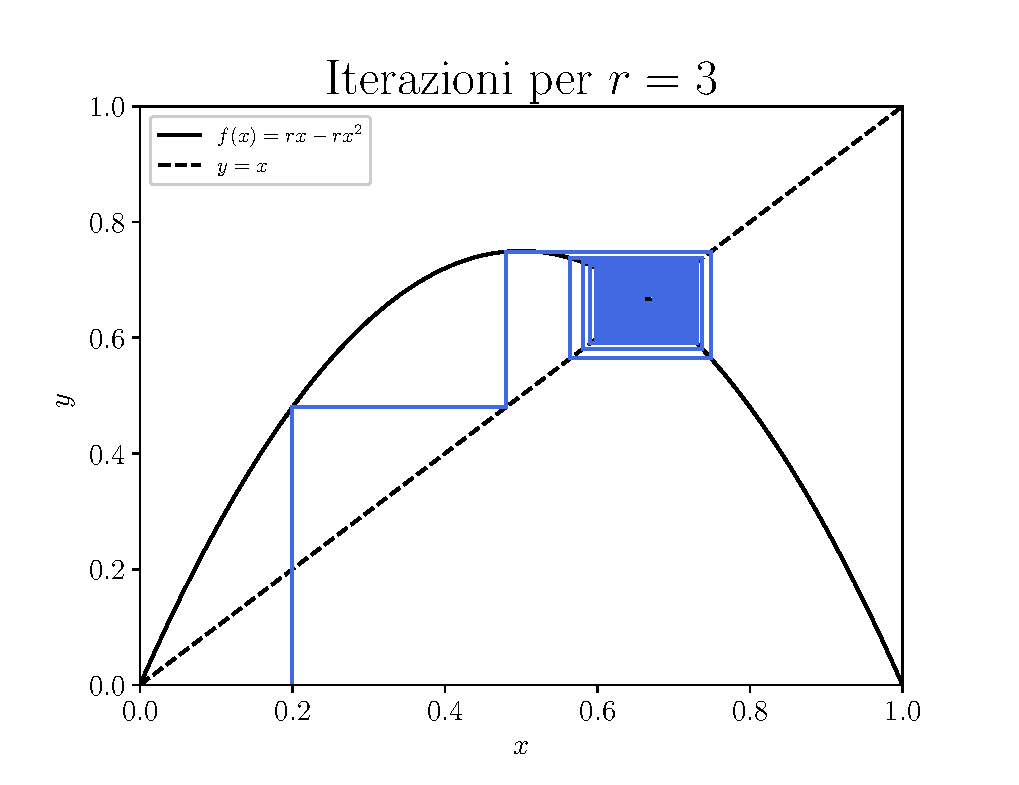
\includegraphics[scale=0.65]{Immagini/iterazioni_r3.eps} 
    \captionsetup{width=.8\linewidth}
    \caption{Iterazioni della funzione logistica per $r=3$. Per non sovraccaricare inultimente il grafico, si è scelto di raffigurare la convergenza a partire da un solo valore iniziale, ma la situazione si ripresenterebbe uguale anche partendo da un qualsiasi altro valore. Si nota come la convergenza attorno a $x_{eq,2}$ sia molto lenta, in particolare come il punto di equilibrio e lo stato del sistema dopo 1000 iterazioni siano ancora distinguibili sulla scala visualizzata, al contrario di figure precedenti.}
    \label{fig:r3}
    \end{center}   
\end{figure}

Ricapitolando il risultato di questi due ultimi paragrafi, si è trovato che quando $r$ è inferiore a 1 la popolazione è irrimediabilmente destinata a estinguersi, a prescindere dal valore iniziale. Quando $r$ invece diventa maggiore di 1, ma inferiore o uguale a 3, la popolazione cresce a partire da valori iniziali piccoli, o decresce a partire da valori iniziali grandi, fino a raggiungere asintoticamente il valore $1-1/r$, per mantenersi stabile in questo stato. Per $r=3$, tuttavia, la convergenza risulta estremamente lenta. Come si vedrà adesso, la situazione cambia radicalmente per $r > 3$.

\subsection{Punti fissi per $3 < r \leq 4$: verso il caos}
\begin{figure}[h!]
    \begin{center}
        \subfigure[]{\label{fig:osc_a} 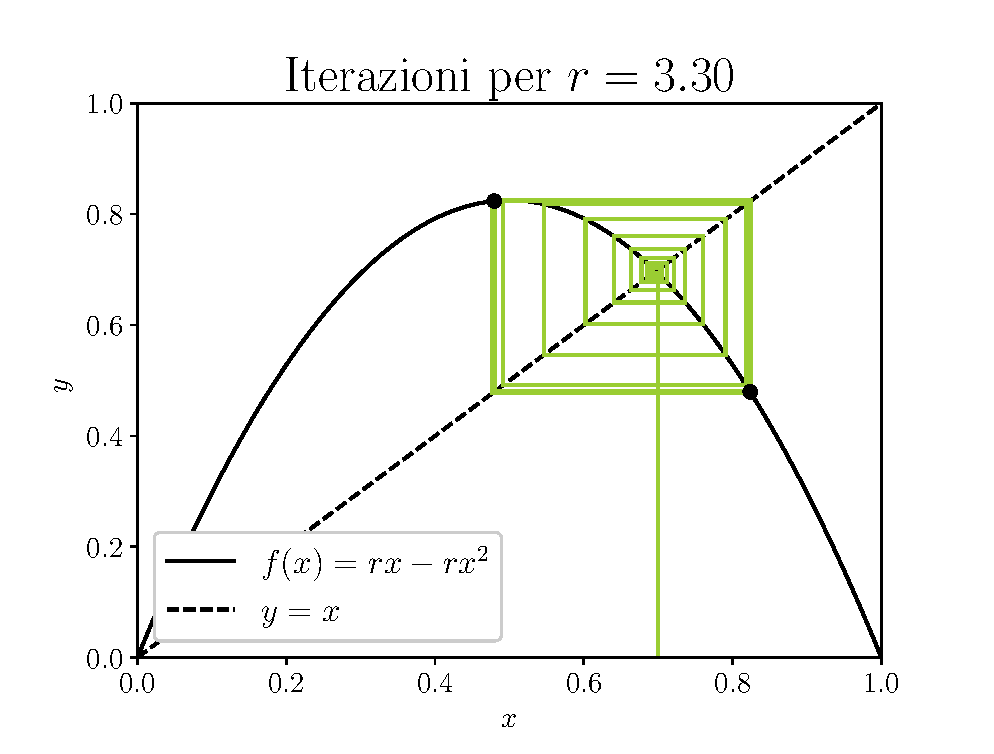
\includegraphics[scale=0.45]{Immagini/oscillazioni_1.eps}}
        \subfigure[]{\label{fig:osc_b} 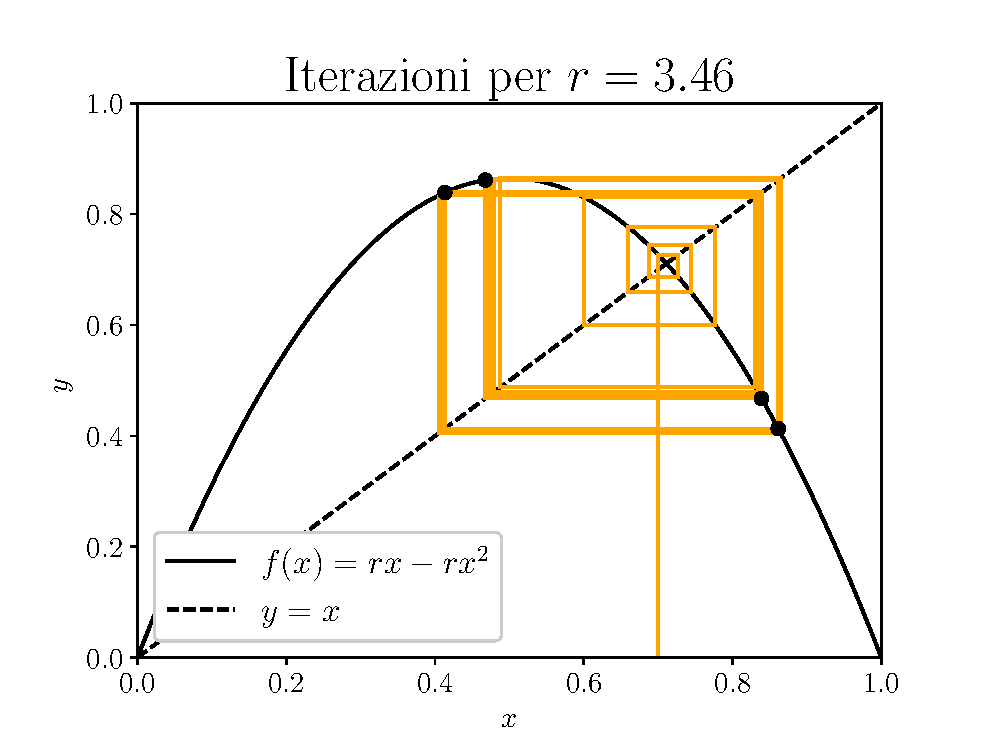
\includegraphics[scale=0.45]{Immagini/oscillazioni_2.eps}}
        \subfigure[]{\label{fig:osc_c} 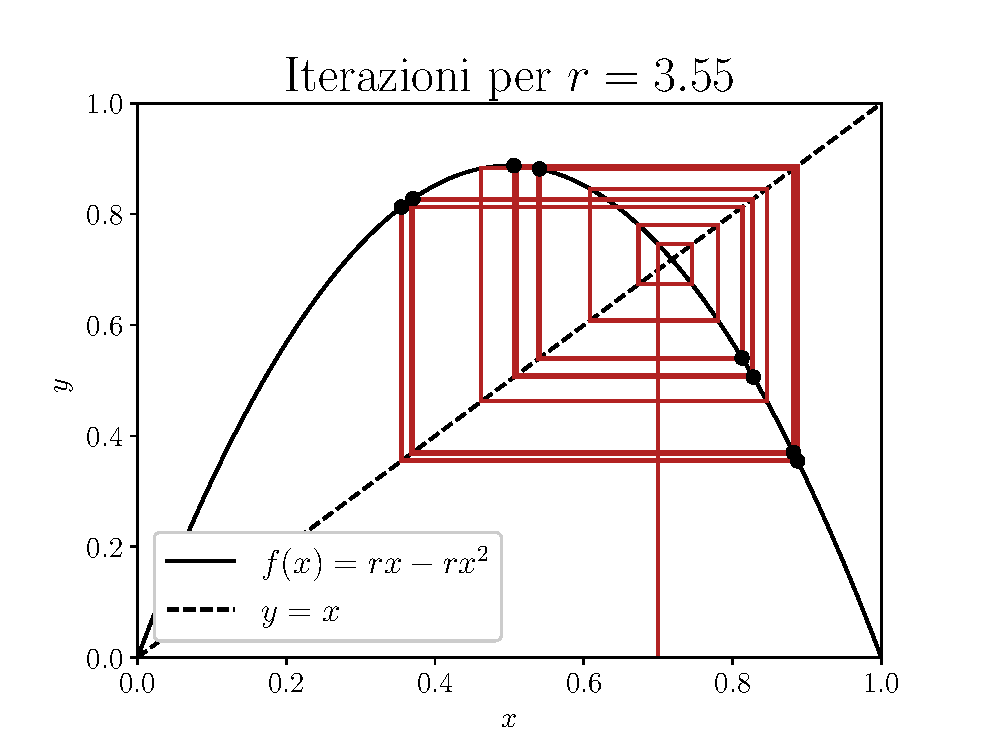
\includegraphics[scale=0.45]{Immagini/oscillazioni_3.eps}}
        \captionsetup{width=.8\linewidth}   
    \caption{Per $r > 3$ il sistema non evolve più convergendo a un valore, ma oscilla tornando periodicamente sugli stessi punti, il cui numero dipende dal valore di $r$. Nelle tre figure sono stati rappresentati, nell'ordine, i casi in cui il sistema oscilla tra 2, 4 e 16 valori. Si sono fatte partire le iterazioni dallo stesso valore, $0.7$.}
    \label{fig:oscillazioni}
    \end{center}
\end{figure}

Per $3 < r \leq 4$, sfruttando i calcoli effettuati selle sezioni precedenti, si ottiene che sia $x_{eq,1}$ che $x_{eq,2}$ sono punti fissi repulsori. Cosa succede quindi alla popolazione, se sembra che non ci siano dei valori a cui essa può tendere asintoticamente? In realtà, ci si rende conto che esistono dei punti fissi per la cosiddetta \textit{iterata seconda} di $f$, vale a dire 
\begin{equation*}
f^2(x) := f(f(x)) = r^2 x (1-x) (rx^2 -rx +1)
\end{equation*}
La funzione $f^2(x)$ è una quartica e ha quattro punti fissi, vale a dire soluzioni dell'equazione 
\begin{equation*}
    f^2(x) = x \quad \Rightarrow \quad x (r^2 (1-x) (rx^2 -rx +1) - 1) = 0
\end{equation*}
Due soluzioni sono ovviamente $x_{eq,1}$ e $x_{eq,2}$ viste fin'ora, le altre due invece sono 
\[
    \boxed{x_{eq,3,4} = \dfrac{r +1 \pm \sqrt{r^2 -2r -3}}{2r}}
\]
Calcolando la derivata di $f^2(x)$, si trova che nei due punti $x_{eq,3,4}$ la derivata assume lo stesso valore, il quale può essere, in modulo, sia maggiore che minore di 1 per $ 3 < r \leq 4$. 

Consideriamo prima il caso in cui la derivata risulti in modulo minore di 1, e quindi ci siano punti fissi attrattori per $f^2$. Si calcola che questa situazione si verifica per tutte le $r$ tali che $$ 3 < r \leq 1 +\sqrt{6}$$
Chiamiamo $r_1 := 1 +\sqrt{6} \simeq 3.449$. Dal punto di vista dell'evoluzione del sistema, queste due soluzioni rappresentano degli stati tra i quali il sistema, dopo infinite iterazioni, continua a oscillare, tornando su ciascuno di essi ogni due iterazioni di $f$: se a un certo istante il sistema si trova in corrispondenza di $x_{eq,3}$, all'iterazione successiva si troverà in $x_{eq,4}$, alla successiva di nuovo in $x_{eq,3}$, e così via. Il fatto che essi siano attrattori indica che il sistema, partendo da un certo valore iniziale, evolve tendendo asintoticamente a oscillare tra essi. Tale comportamento è visibile graficamente nella figura \ref{fig:osc_a}.


Quando invece $r_1 < r \leq 4$ la derivata di $f^2$ in $x_{eq,3,4}$ diventa maggiore di 1, e questi punti diventano quindi fissi repulsori; il sistema non evolve più tendendo a oscillare tra essi asintoticamente. Si verifica però che esistono 4 nuovi punti fissi per l'\textit{iterata terza} di $f$, $f^3$, che risultano attrattori però solo per valori di $r$ compresi tra $r_1$ e un nuovo valore $r_2 \simeq 3.544$. Per tali valori di $r$, all'infinito il sistema oscilla periodicamente tra i 4 punti fissi di $f^3$, tornando su ciascuno di essi ogni 4 iterazioni di $f$: si dice che il \textit{periodo di oscillazione} è pari a 4.

Quando $r$ supera il valore $r_2$, i quattro punti trovati diventano instabili, ma si trovano 8 nuovi punti fissi per l'iterata quarta di $f$, $f^4$, tra i quali il sistema oscilla, stavolta con periodo 8, fintanto che tali punti risultano attrattori di $f^4$, ovvero per $r$ maggiore di $r_3$ e minore di un certo altro valore $r_4$. Dopodiché sorgono 16 nuovi punti fissi per $f^5$, attrattori fino a un altro valore $r_5$, poi altri 32 punti fissi per $f^6$, e avanti così, con il numero dei punti fissi e la lunghezza del periodo di oscillazione che crescono esponenzialmente con le potenze del 2. Questa situazione è visibile nella figura \ref{fig:oscillazioni}, dove sono state raffigurate le oscillazioni del sistema attorno ai punti di equilibrio delle iterate di $f$ per diversi valori di $r$.


\subsection{Comportamento per $r > r_c$: il caos}
La situazione appena descritta continua finché non si raggiunge un valore critico di $r$ circa pari a 
\[
    \boxed{r_c \simeq 3.56995}
\]
Quando $r>r_c$, il sistema oscilla tra infiniti valori tutti diversi tra loro, tra i quali è impossibile riconoscere una periodicità. Inoltre, pur partendo da valori iniziali arbitrariamente vicini tra loro, non è possibile ottenere evoluzioni che rimangano arbitrariamente vicine anche dopo infinite iterazioni: le due evoluzioni, dopo una certa iterazione, saranno completamente differenti, rendendo la predizione dell'evoluzione estremamente dipendente dal valore iniziale. 
\begin{minipage}{\linewidth}
    \makebox[\linewidth]{
    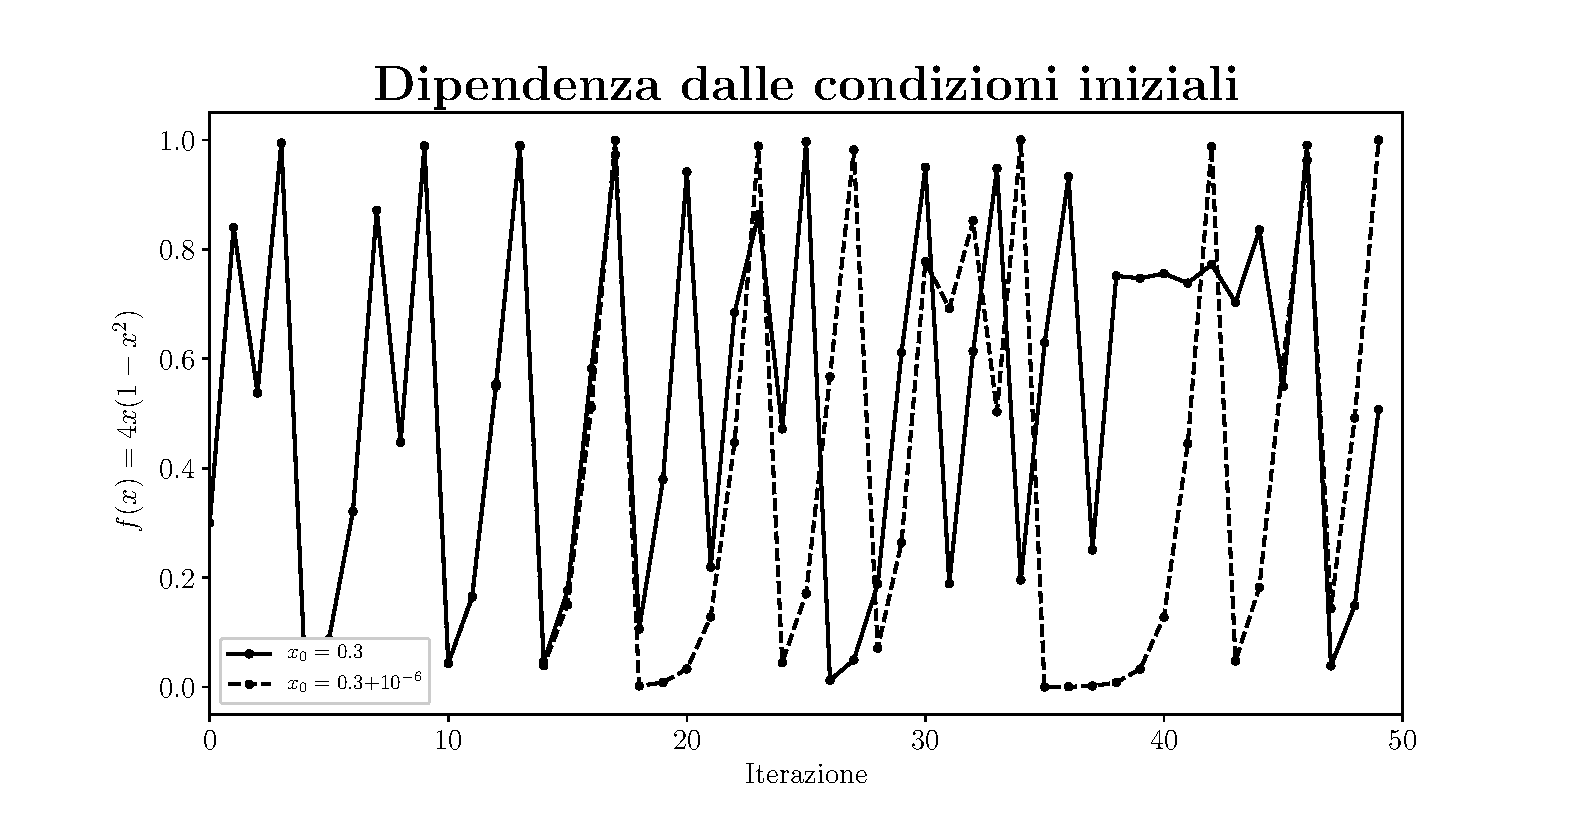
\includegraphics[scale=0.5]{Immagini/caos.eps}}
\end{minipage}   

\captionsetup{width=.8\linewidth}
\captionof{figure}{Sull'asse delle ascisse è riportato il numero dell'iterazione corrente della funzione logistica, sull'asse delle ordinate sono riportati gli stati alla $k$-esima iterazione di due evoluzioni partite una dal valore $x_0$, l'altra dal valore $x_0 + \epsilon$, dove si è scelto in questo caso $\epsilon = 10^{-6}$. Dopo alcune interazioni le due evoluzioni differiscono fortemente e non si trova più alcuna analogia tra esse.}
\label{fig:caos}
\vspace{20pt}

Questo fenomeno, vale a dire la forte dipendenza dai valori iniziali, è una delle caratteristiche principali dei fenomeni caotici, che di solito, quando insorgono, sono legati a dinamiche descritte da equazioni non lineari, come è infatti l'equazione logistica. Un esempio per visualizzare la forte dipendenza del sistema dalle considizioni iniziali è rappresentato nella figura \ref{fig:caos}, dove si sono scelti due valori iniziali distanti $\epsilon$ piccolo a piacere (nella figura $\epsilon = 10^{-6}$), e si sono tracciate le evoluzioni dell'equazione logistica a partire da essi. Si vede chiaramente che, dopo una decina di iterazioni, le due evoluzioni iniziano a differire sensibilmente, evolvendo in modo del tutto diverso. Tale comportamento è tanto più accentuato quanto più $r$ si avvicina al valore 4, ovvero evoluzioni che partono da valori molto vicini iniziano a divergere tanto prima, quanto più il valore di $r$ è grande.



\subsection{Non solo caos: isole di periodicità}
\begin{figure}[h!]
    \begin{center}  
    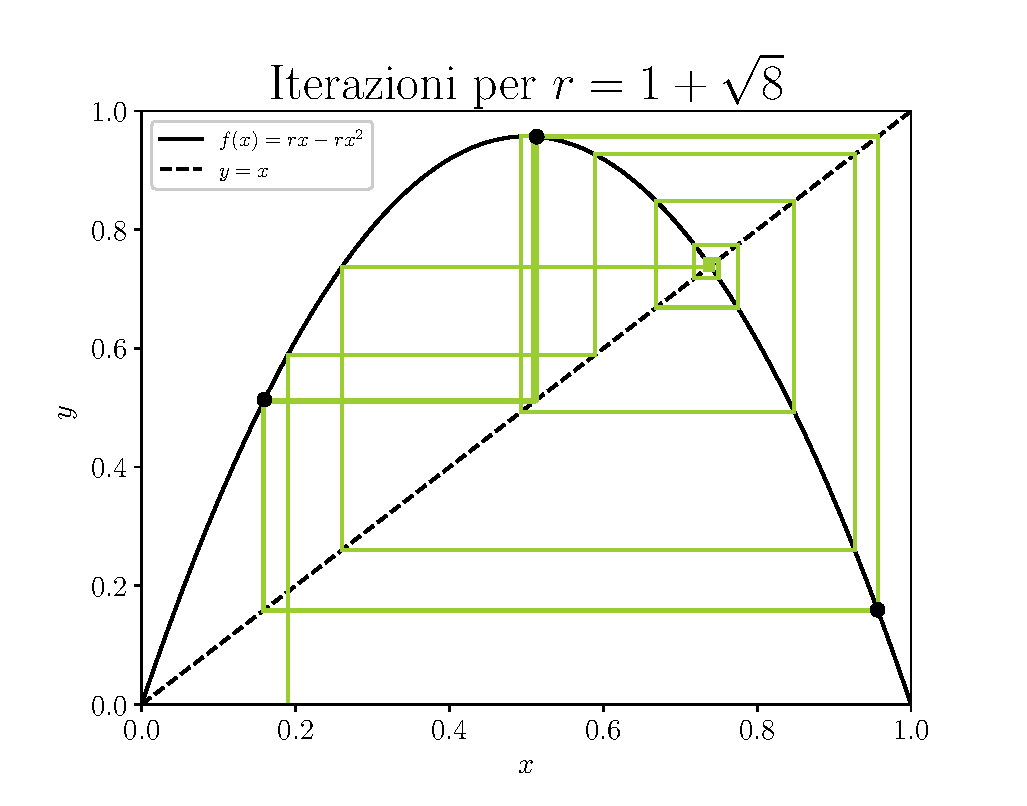
\includegraphics[scale=0.6]{Immagini/3_oscillazioni.eps} 
    \captionsetup{width=.8\linewidth}
    \caption{Oscillazione del sistema tra tre valori. Si può osservare che per $r = 1 + \sqrt{8}$, dopo un certo numero di iterazioni iniziali il sistema si assesta a oscillare tra 3 valori, che sono quelli sul grafico di $f$ per cui la linea verde risulta più spessa.}
    \label{fig:tre_osc}
    \end{center}   
\end{figure}
Si può pensare che, superato il valore $r_c$, il comportamento della mappa logistica continui semplicemente a essere caotico, ma in realtà si trova un altro fenomeno davvero interessante: per certi valori di $r$ si trova che la mappa logistica ritorna a oscillare periodicamente, ma stavolta non tra $2^k$ stati, bensì tra un numero dispari di stati. Ad esempio, per $r = 1 + \sqrt{8}$ il sistema oscilla periodicamente tra 3 valori, come mostrato dalla figura \ref{fig:tre_osc}.

In realtà un teorema, detto \textit{teorema di Sharowskii}, prevede che per ogni $N \in \mathbb{N}$ esista un valore di $r$ ammissibile per il quale il sistema oscilla tra $N$ valori. In pratica, quindi, nell'intervallo tra $r_c$ e 4 il caos è inframezzato da infinite "isole di periodicità", nelle quali il sistema torna ad assumere un carattere oscillatorio, ogni volta tra un numero diverso di stati. È assai celebre la rappresentazione grafica di questo comportamento nel cosiddetto "albero di Feigenbaum", nel quale vengono rappresentati sulle ascisse i valori che può assumere $r$, mentre sulle ordinate i valori asintotici del sistema dopo un numero infinito di iterazioni. Se il sistema ha un solo punto fisso attrattore, nel grafico sarà presente un solo punto, come si osserva infatti per $r<3$, mentre se il sistema oscilla tra più stati diversi, si fa "dividere" il grafico tra di essi. Il risultato è rappresentato nella figura \ref{fig:feigenbaum}.

\begin{minipage}{\linewidth}
\makebox[\linewidth]{
    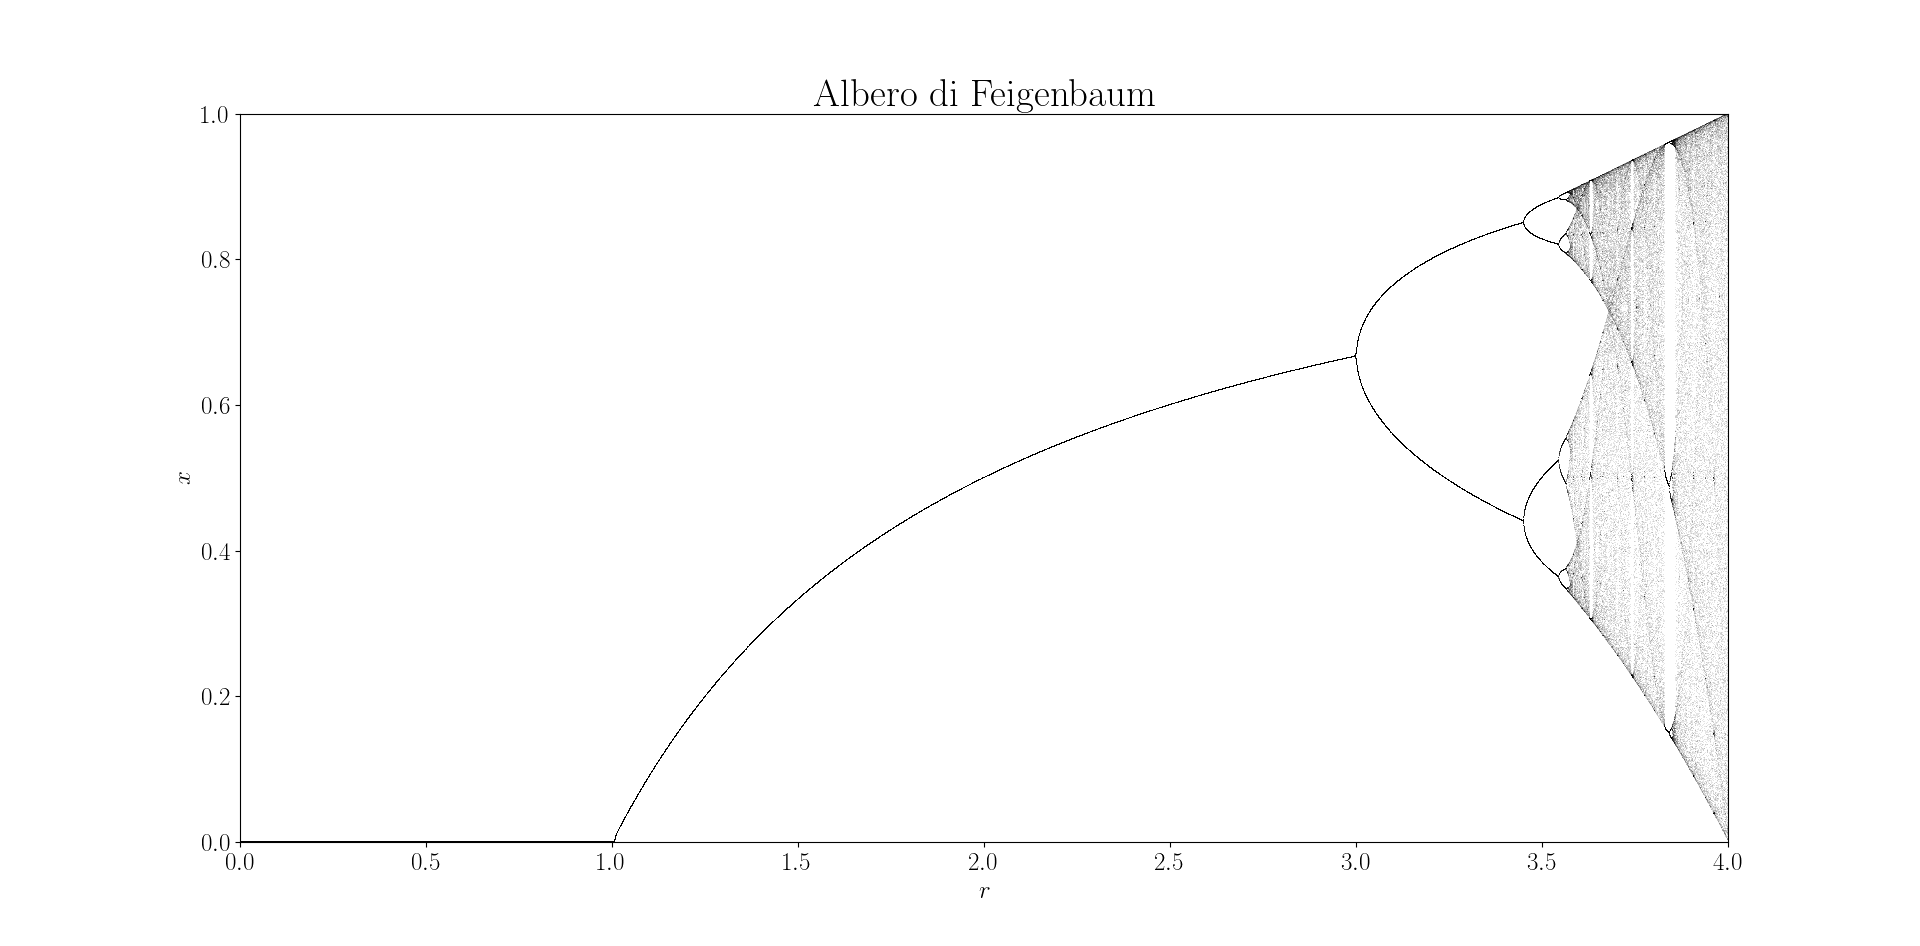
\includegraphics[scale=0.35]{Immagini/feigenbaum.png}}
\end{minipage}
\captionsetup{width=.8\linewidth}
    \captionof{figure}{L'albero di Feigenbaum rappresenta sulle ascisse i valori di $r$ e sulle ordinate i valori asintotici del sistema. Gli sdoppiamenti del grafico indicano che il sistema passa dal convergere a un valore all'oscillare tra più valori. Come si nota, dopo $r=3$ il sistema inizia a raddoppiare il proprio periodo di oscillazione fino al valore $r_c \simeq 3.56995$. Dopo di questo, però, si trovano ancora degli stati oscillatori, come quello molto ben visibile tra tre stati, per $r \simeq 1.8$.}
    \label{fig:feigenbaum}

\vspace{30pt}
\section{Conclusioni}
Lo studio dell'equazione logistica come modello per descrivere la dinamica di una popolazione ha messo in luce quanto l'evoluzione di un sistema possa essere resa complessa semplicemente rendendo quadratica un'equazione lineare. Nonostante le equazioni in gioco per risolvere la dinamica siano facilmente risolvibili analiticamente, la complessità dell'evoluzione può essere spinta al punto da dare origine a dinamiche caotiche, caratterizzate da una forte dipendenza dei valori iniziali e in cui non è possibile trovare una convergenza asintotica. È interessante però notare che la non linearità dell'equazione logistica non implica che l'evoluzione sia sempre di carattere caotico; in molti casi infatti la dinamica si risolve in casi di convergenza asintotica molto semplice da analizzare. 
\vspace{30pt}
\section*{Note finali}
I grafici e le simulazioni presentati in questo documento sono stati realizzati realizzati in Python e i sorgenti sono disponibili, assieme al sorgente \LaTeX di questo stesso documento, presso \url{https://github.com/elenaacinapura/Mappa_Logistica}
\vspace{30pt}
\section*{Bibliografia}
\begin{itemize}
    \item \textit{Moti ordinati e moti caotici nelle mappedell’intervallo in sé, ed applicazioni}, tesi di laurea triennale in Fisica di Federico Gasparotto, presso l'università di Padova. Link: \url{http://tesi.cab.unipd.it/46532/1/Gasparotto_Federico.pdf}
    \item \textit{Appunti sulla mappa logistica} di Fabio ruini, Ph.D. in Economia presso l'università di Modena e Reggio Emilia. Link: \url{http://www.fabioruini.eu/unimore/ttps/Mappa%20logistica.pdf}
    \item Appunti sulle \textit{Traiettorie periodiche} nel contesto del corso di Sistemi Ecologici, di Ettore Fornasini, professore ordinario presso l'università di Padova. Link: \url{http://www.dei.unipd.it/~fornasini/SE_traccia_11_.pdf}
    \item Slides sulla mappa logistica di Simone Zuccher, Ph.D. presso l'università di Verona. Link: \url{http://profs.sci.univr.it/~zuccher/downloads/zuccher-logistica20130503.pdf}
\end{itemize}
\end{document}